% !TEX TS-program = xelatex
% !TEX encoding = UTF-8 Unicode
\documentclass[11pt,a4paper,twoside]{book}
\usepackage{amsmath,amssymb}
\usepackage{empheq}
\usepackage[semibold]{ebgaramond}
\usepackage[cmintegrals,cmbraces]{newtxmath}
\usepackage{ebgaramond-maths}
\usepackage{bm}
\usepackage[OMLmathrm, OMLmathsfit, rmdefault=mdugm]{isomath}
\usepackage{tocbibind}
\usepackage{makeidx}
\makeindex

\makeatletter
  \DeclareSymbolFont{ntxletters}{OML}{ntxmi}{m}{it}
  \SetSymbolFont{ntxletters}{bold}{OML}{ntxmi}{b}{it}
  \re@DeclareMathSymbol{\leftharpoonup}{\mathrel}{ntxletters}{"28}
  \re@DeclareMathSymbol{\leftharpoondown}{\mathrel}{ntxletters}{"29}
  \re@DeclareMathSymbol{\rightharpoonup}{\mathrel}{ntxletters}{"2A}
  \re@DeclareMathSymbol{\rightharpoondown}{\mathrel}{ntxletters}{"2B}
  \re@DeclareMathSymbol{\triangleleft}{\mathbin}{ntxletters}{"2F}
  \re@DeclareMathSymbol{\triangleright}{\mathbin}{ntxletters}{"2E}
  \re@DeclareMathSymbol{\partial}{\mathord}{ntxletters}{"40}
  \re@DeclareMathSymbol{\flat}{\mathord}{ntxletters}{"5B}
  \re@DeclareMathSymbol{\natural}{\mathord}{ntxletters}{"5C}
  \re@DeclareMathSymbol{\star}{\mathbin}{ntxletters}{"3F}
  \re@DeclareMathSymbol{\smile}{\mathrel}{ntxletters}{"5E}
  \re@DeclareMathSymbol{\frown}{\mathrel}{ntxletters}{"5F}
  \re@DeclareMathSymbol{\sharp}{\mathord}{ntxletters}{"5D}
  \re@DeclareMathAccent{\vec}{\mathord}{ntxletters}{"7E}
\makeatother

\usepackage{array}
% to produce a comma between multiple footnotes / https://tex.stackexchange.com/questions/40072/incompatibility-between-footmisc-option-multiple-and-hyperref/62091#62091
\let\oldFootnote\footnote
\newcommand\nextToken\relax
\renewcommand\footnote[1]{%
    \oldFootnote{#1}\futurelet\nextToken\isFootnote}
\newcommand\isFootnote{%
    \ifx\footnote\nextToken\textsuperscript{,}\fi}

\defaultfontfeatures{Ligatures=TeX} % makes this a feature for all selected fonts
\usepackage{esint}
\usepackage{polyglossia}
\setmainlanguage{english}
\usepackage[text={18cm,26cm},centering]{geometry} % 
\usepackage{natbib}
\usepackage{graphicx}
\graphicspath{{pics/}}
\usepackage[usenames,dvipsnames,svgnames,table]{xcolor}
\usepackage{hyperref}
\usepackage{url}
\usepackage[export]{adjustbox}

\hypersetup{
  colorlinks,
  citecolor=bleuSU,
  linkcolor=bleuSU
}
\definecolor{bleuSU}{RGB}{26,39,101}

\usepackage[normalem]{ulem}
\makeatletter
\renewcommand*{\uuline}{%
  \bgroup
  \UL@setULdepth
  \markoverwith{%
    \lower\ULdepth\hbox{%
      \kern-.03em%
      \vtop{%
        \hrule width.2em%
        \kern 0.6pt % distance between the two underlines
        \hrule
      }%
      \kern-.03em%
    }%
  }%
  \ULon
}
\makeatother
\setlength{\ULdepth}{-2pt}  % distance from double underline to letter

\newcommand{\delS}{\delta S}
\newcommand{\delA}{\delta A}
\newcommand{\delh}{\delta h}
\newcommand{\delt}{\delta t}
\newcommand{\delz}{\delta z}
\newcommand{\delbx}{\delta \matrixsym x}
\newcommand{\lp}{\left(}
\newcommand{\rp}{\right)}
\newcommand{\itA}{\textit A}
\newcommand{\itB}{\textit B}
\newcommand{\dAB}{\mathcal D_{AB}}
\newcommand{\bA}{\matrixsym A}
\newcommand{\bff}{\matrixsym{f}}
\newcommand{\bF}{\matrixsym{F}}
\newcommand{\bj}{\matrixsym{j}}
\newcommand{\bJ}{\matrixsym J}
\newcommand{\bn}{\matrixsym{n}}
\newcommand{\bN}{\matrixsym N}
\newcommand{\bp}{\matrixsym{p}}
\newcommand{\bP}{\matrixsym{P}}
\newcommand{\br}{\matrixsym r}
\newcommand{\bt}{\matrixsym t}
\newcommand{\be}{\matrixsym e}
\newcommand{\bu}{\matrixsym u}
\newcommand{\bv}{\matrixsym v}
\newcommand{\bw}{\matrixsym w}
\newcommand{\bx}{\matrixsym x}
\newcommand{\pd}[2]{\frac{\partial #1}{\partial #2}}
\newcommand{\D}[2]{\frac{D #1}{D #2}}
\newcommand{\dd}[2]{\frac{\mathrm d #1}{\mathrm d #2}}
\newcommand{\dA}{\mathrm dA}
\newcommand{\dV}{\mathrm dV}
\newcommand{\dS}{\mathrm dS}
\newcommand{\prg}[1]{\paragraph{$\rhd$ #1}}
\newcommand{\alphaijkl}{\alpha_{ijkl}}
\newcommand{\Aijkl}{A_{ijkl}}
\newcommand{\delij}{\delta_{ij}}
\newcommand{\sigij}{\sigma_{ij}}
\newcommand{\sigji}{\sigma_{ji}}
\newcommand{\sigxy}{\sigma_{xy}}
\newcommand{\matL}{\mathcal L}
\newcommand{\matO}{\mathcal O}
\newcommand{\matS}{\mathcal S}
\newcommand{\kij}{k_{ij}}
\newcommand{\tensor}[1]{\smash{\uuline{#1}{}}}
\setlength{\parindent}{0pt} % remove indent
  
\begin{document}
{
\title{\textit{Physics of fluids \& nonlinear physics}}
%\author{Arnaud Antkowiak \qquad Camille Duprat}
\author{
  Arnaud Antkowiak\footnote{\href{mailto:arnaud.antkowiak@upmc.fr}{arnaud.antkowiak@upmc.fr}}
  \and
  Camille Duprat\footnote{\href{mailto:camille.duprat@ladhyx.polytechnique.fr}{camille.duprat@ladhyx.polytechnique.fr}}
}
\date{v0.21.09$_\text{12}$}
\maketitle
\tableofcontents
}
% !TEX root = ./physics_of_fluids.tex
% !TEX TS-program = xelatex
% !TEX encoding = UTF-8 Unicode
\newpage
\section*{Modelling fluids}
\chapter{Fluid motion}
\label{chap:fluid-motion}
%Note : cours fait en 2019-2020 sur 2h30 à fond les manettes
The description of fluid flows can rapidly be obscured behind seemingly complex equations (e.g. Navier--Stokes). Even worse these equations can change depending on the context and problem considered. Actually, the governing equations for fluid motion express truly simple physical principles, namely \textbf{mass conservation} (the mass $m(t)$ of a fluid particle is constant), \textbf{momentum conservation} (a fluid particle's momentum obeys Newton's second law $m \matrixsym \gamma = \Sigma \bF$) and \textbf{energy conservation} (the energy of a fluid particle follows the first and second principle of thermodynamics).  In this introduction we will review the derivation of the fluid mechanics equations by expressing these fundamental conservation principles.
\section{Forces}
As other continuum media, fluids carry force fields that determine their equilibrium (when the net force contribution is zero) or their motion. If each fluid particle is subject to \textit{body forces}, it is also exposed to \textit{surface forces} called \textbf{stresses}, as for example pressure~(Fig.~\ref{fig:weather_map}) that we now examine.
\begin{figure}[htbp]
\begin{center}
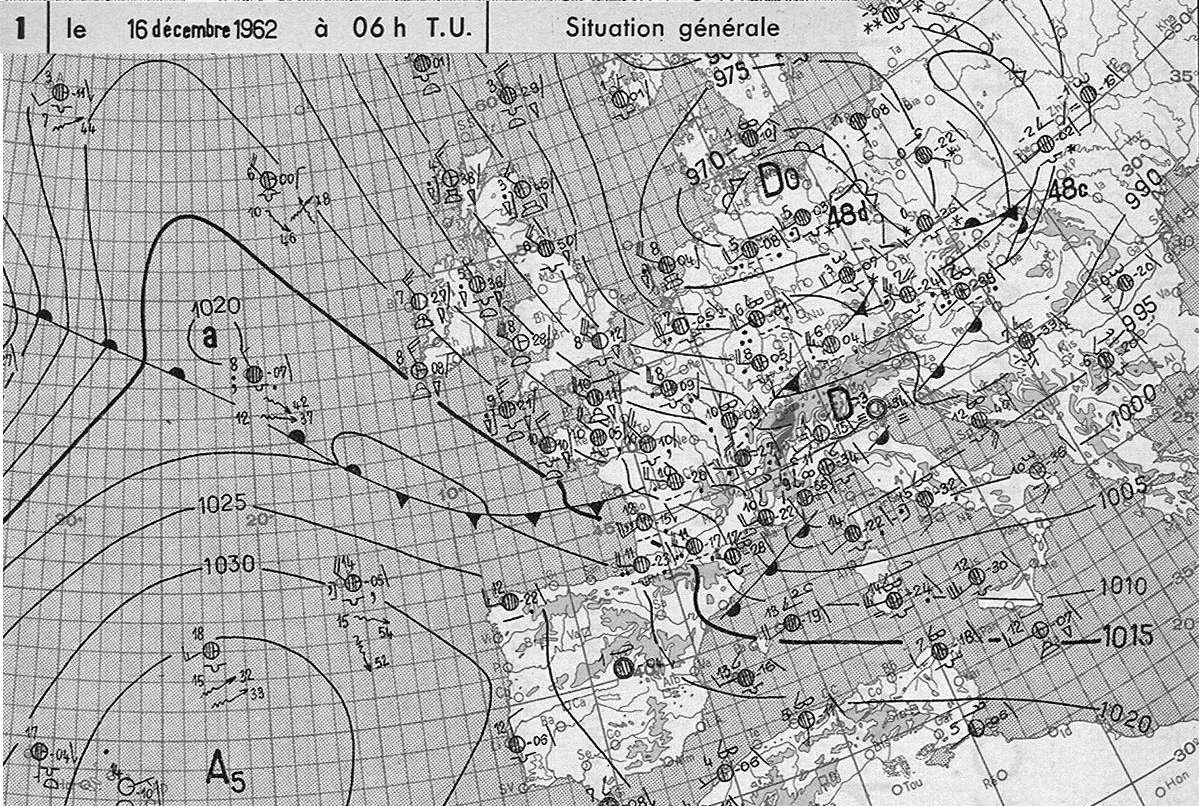
\includegraphics[height=5cm]{19621216Surface.jpg}
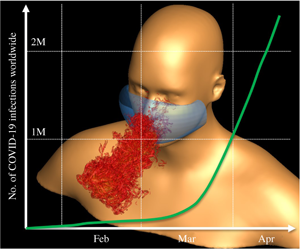
\includegraphics[height=5cm]{covid.png}
\caption{\textbf{Illustrations of pressure forces in daily-life phenomena.} Left: France isobaric map from December, 16 1962. The map reveals low-pressure area and anticyclones (high-pressure area). The clustering isobars near Corsica are a signature of the violent winds that swept the region (force 12 on the Beaufort scale i.e. the threshold for hurricanes for sailors ; 216 km/h at the cap Corse). Source: \url{http://tempetes.meteo.fr}. Right: a coughing event is associated with a violent lung compression. The resulting overpressure drives a rapid airflow that may torn and transport liquid droplets and aerosols \citep{Mittal2020}.}
\label{fig:weather_map}
\end{center}
\end{figure}

\subsection{Pressure}
\prg{Archimedes\index{Archimedes principle} principle without equation.} Consider a fluid at equilibrium in the gravity field (Fig.~\ref{fig:archimedes}). Let's isolate now mentally a fluid portion. It experiences from the gravity field a force corresponding to its \textit{weight}  $\bP$ pointing downwards. It also bears \textit{pressure forces} from the surrounding fluid. Since the fluid portion is at equilibrium, the net pressure force has to balance the weight (equal in intensity but opposite in direction). Now if in our mind experiment we were to replace the fluid portion by a solid object, the resulting action of the external forces would not change: the net force exerted by pressure forces is still equal in intensity to the weight of the fluid ``displaced'' by the solid. The resultant of pressure forces corresponds to the \textit{buoyancy} \citep{Lighthill1986}. Of course if the solid is denser (or less dense) than the surrounding fluid, the equilibrium would be lost and fluid/body motion would set in.

\noindent Pressure is a force per unit surface which is \textbf{normal} to the considered surface\footnote{We may see this feature as the \textit{definition} of a fluid, i.e. a medium unable to resist shear \citep{Prandtl1957}. A shear stress would therefore unvariably set the fluid into motion. Actually \citet[][\S1.3]{Batchelor1967} argue that if the pressure force would not be aligned with the normal vector, equilibrium could not be achieved.}. This type of distributed force in a fluid is a specificity of continuum media, and is referred to as \textbf{stress}. Here the corresponding stress expression is therefore:
\begin{equation}
\mathrm d \bff = -p \,\bn \,\dS.
\label{eq:pressure_stress}
\end{equation}
The minus sign translate the state of compression in which fluids generally are (so that pressure is a positive quantity, unless in very specific cases of tensile solicitations of fluids).
\prg{Pressure as a body force.} On figure~\ref{fig:pressure_gradient} we illustrate the action of pressure forces exerted on a small cylindrical fluid portion. The portion has a base $S$ and a height $\mathrm dn$ leaning on two isobars $p$ and $p+\mathrm dp$. The action of pressure forces on the side of the cylinder is zero by symmetry, so that the net pressure force is simply the sum of the contributions exerted on each bounding face : $S\,p$ and $-S\,\lp p+\mathrm dp\rp$ (let's count positively -- and arbitrarily -- the forces oriented along the pressure gradient), which is $-S \,\mathrm dp$. If we divide this force by the volume of the small element, $S \, \mathrm dn$, it appears that pressure forcescan be perceived as a body force of intensity $-\pd{p}{n}$ acting along $\nabla p$. In other words pressure forces may be understood as body forces of intensity $-\nabla p$; this is the meaning of this term appearing in both Euler and the Navier--Stokes equations.
\begin{figure}[htbp]
\begin{center}
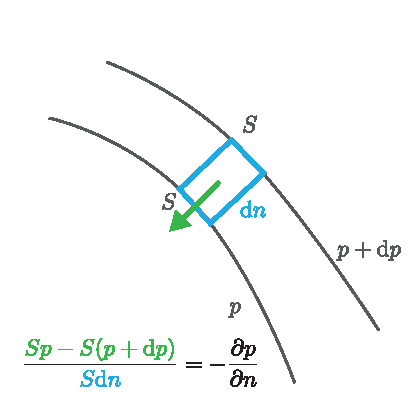
\includegraphics[page=1,width=5cm]{./pics/pressure_gradient.pdf}
\caption{Writing down a force balance on a volume portion $S\,\mathrm dn$ leaning on two isobars (of level $p$ and $p + \mathrm dp$), we see that the pressure action may be understood as a body force per unit volume of intensity~$-\pd{p}{n}$.}
\label{fig:pressure_gradient}
\end{center}
\end{figure}
This is here a physical interpretation of the divergence theorem which would have given directly:
$$
-\iint_{\partial V} p \,\bn \, \dS = -\iiint_V \nabla p \,\dV.
$$

\subsection{Stresses}
\begin{figure}[htbp]
\begin{center}
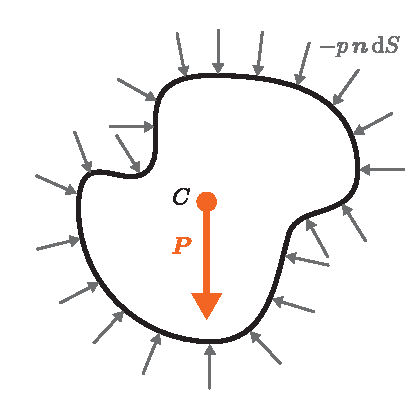
\includegraphics[page=1,width=5cm]{./pics/01_pics.pdf}\qquad\includegraphics[page=2,width=5cm]{./pics/01_pics.pdf}
\caption{Left: when at equilibrium in the gravity field, every fluid portion experiences pressure forces that exactly balance the weight action $\bP$. Right: the pressure stress is normal to each surface element.}
\label{fig:archimedes}
\end{center}
\end{figure}
In the general context of a flowing fluid, stress has no particular reason to be aligned with the normal -- and, as a matter of fact, it is not. But multiplying the normal vector $\bn$ with a scalar can only give another vector still aligned with $\bn$, and using the cross product is of no help either because the cross product between any vector and $\bn$ can only give a vector perpendicular to $\bn$. So we need another mean to obtain a vector arbitrarily oriented from the unique knowledge of $\bn$. The mathematical object allowing to perform this operation is the 2-rank tensor. On using Einstein notations, this gives:
\begin{equation}
\mathrm df_i = \sigij n_j \, \dS.
\end{equation}
We have here to remember that this object is only a mean to obtain $\mathrm d \bff$ not necessarily aligned with $\bn$.

\noindent Of course it is possible to obtain the simple case of a stress aligned with $\bn$ using this formalism. As an example, the stress tensor of a fluid at rest (éq.~\ref{eq:pressure_stress}) is:
\begin{equation}
\sigij = -p\, \delij.
\label{eq:static_stress_tensor}
\end{equation}

\noindent It is possible to show that this stress tensor $\mathsfbfit \sigma$ is necessarily a symmetric tensor, i.e. $\sigij = \sigji$ \citep{Batchelor1967}. The demonstration's main idea is to write an angular momentum balance at the fluid particle level; the only dominant term in this equation involves the antisymmetric part of $\mathsfbfit{\sigma}$. As it is not balanced by any term, it necessarily vanishes. There is one exception however: in the very particular case of a \textit{moment density}, as in active matter or certain magnetic colloids, this term can be balanced and the tensor be non-symmetric \citep[see for example the study of][]{Soni2019}. 
\subsection{Body forces}
\noindent Fluids are also subject to more conventional body forces, which can be magnetic, electrostatic, gravity or result from non-inertial effects (think of centrifuge or Coriolis pseudo-forces). On noting $\bF$ the body force \textbf{per unit mass} acting on the fluid particle level, we can write the net body force exerted on a fluid portion $V$ as:
\begin{equation}
\iiint_V \rho \bF \,\dV.
\end{equation}
\prg{To summarize.} The net force acting on a fluid portion $V$ is the sum of surface and body forces:
\begin{equation}
\oiint_{\partial V} \mathsfbfit \sigma \!\cdot\! \bn\,\dS + \iiint_V \rho \bF \,\dV.
\end{equation}
\section{Fluid equilibrium}
\noindent At equilibrium, pressure and body force exerted on any part $V$ of a fluid balance each other:
$$
\iiint_V \rho \bF \,\dV -\iint_{\partial V} p \, \bn \, \dS = \boldsymbol 0,
$$
or, on using the divergence theorem:
\begin{equation}
\iiint_V \lp \,\rho \bF -\nabla p \rp\,\dV = \boldsymbol 0.
\end{equation}
This relation being verified for \textit{any} fluid domain, we necessarily get at the local level:
\begin{equation}
\rho \bF =\nabla p.
\end{equation}
And we recover here the pressure force expressed as a body force $-\nabla p$.

\textbf{Remark}: Only those density and force fields such that $\rho \bF$ can be expressed as a gradient allow to reach hydrostatic equilibrium (counter-example: the baroclinic instability developing when iso-$p$ differ from iso-$\rho$, or in other words as soons as pressure is not a simple function of $\rho$).
\prg{The case of conservative forces.} Conservative forces derive from the potential $\Psi$:
\begin{equation}
\bF = - \nabla \Psi,
\end{equation}
so that
\begin{equation}
-\rho \nabla \Psi = \nabla p,
\end{equation}
and therefore 
\begin{equation}
\nabla \rho \times \nabla \Psi = \boldsymbol 0.
\end{equation}
The iso-$\rho$ (isopycnals) are then superimposed to equipotentials, themselved superimposed with isobars. \\
\textbf{Consequence}:~in~such~a~system, a free surface corresponding to  $p = 0$ for example will also be an equipotential $\Psi = \text{const}$.

\prg{Example: the equilibrium of a rotating fluid.} Let's consider a rotating container filled with liquid. The container rotates at angular velocity $\Omega$ in the gravity field (the axis of rotation is vertical, i.e. directed along  $\matrixsym e_{z}$). In the rotating frame, each fluid particle experiences gravity but also the centrifuge pseudo-force:
\begin{equation}
\bF_\text{cent} = -\rho \,\matrixsym \Omega \times \lp \matrixsym  \Omega \times \matrixsym r\rp.
\end{equation}
Here $\matrixsym \Omega = \Omega \,\matrixsym e_{z}$. We can then write:
\begin{equation}
\bF_\text{cent} = \rho \Omega^2 r \,\matrixsym e_{r} = -\rho \nabla \Psi_\text{cent},
\end{equation}
where
\begin{equation}
\Psi_\text{cent} = -\frac{1}{2} \Omega^2 r^2 = -\frac{1}{2} \Omega^2 \lp x^2 + y^2\rp.
\end{equation}
Adding gravity effects with $\Psi_\text{grav} = gz$ we get 
\begin{equation}
\Psi_\text{tot} = \Psi_\text{grav} + \Psi_\text{cent}  = gz -\frac{1}{2} \Omega^2 \lp x^2 + y^2\rp.
\end{equation} 
We here remark that the equipotentials are paraboloids. As a result the free surface characterised with $p = 0$\footnote{see chapter~\ref{chap:boundary_conditions} for a discussion of the hypotheses behind this boundary condition.} will also adopt a paraboloidal shape:
\begin{equation}
z_\text{surf} = \frac{1}{2} \frac{\Omega^2}{g} r^2 + \text{const}.
\end{equation}
\prg{Exercise: fluid planet equilibrium.} Consider a self-gravitating fluid sphere. The gravity force per unit masse $\bF$ exerted on each fluid particle derives from the gravity potential $\Psi$ such that:
\begin{equation}
\nabla^2 \Psi = 4 \mathrm \pi \mathcal G \rho,
\end{equation}
where $\mathcal G$ is the universal gravitational constant. With the help of the hydrostatic equation, and supposing that the fluid has a constant density\footnote{This is a really crude approximation on the density profile, which better describes incompressible (!) planets rather than gaseous ones or stars. The hydrostatics of stars can however be rationalised by taking into account the state law of polytropes, and possibly the radiation pressure adding up to the kinetic pressure. The reader interested in stellar hydrostatics may look at the \textit{Lane-Emden equation} described e.g. in \citet[][chap. IV]{Chandrasekhar1957}.} $\rho_0$, show that the radial pressure profile satisfies:
\begin{equation}
p(r) = \tfrac{2}{3} \mathrm \pi \mathcal G \rho_0^2 \lp R^2 - r^2\rp,
\end{equation}
with $R$ the planet radius.
\section{Fluid motion}
Now that we have described the forces at play in a fluid and the conditions for equilibrium, let's focus on fluid motion. 

One technical issue with the simple conservation laws mentioned at the beginning of the chapter is that they are expressed at the fluid particle level. This seems quite natural, but it conflicts with our usual representation of space. Let's clarify what we mean by this by considering a typical fluid flow, for example the one around an airplane wing. Typically we are interested in estimating the forces exerted by the flowing fluid on a the plane, and this requires to build a knowledge of the stresses exerted on the wing. The pressure applied at one given point of the wing is ultimately a consequence of the conservation laws evoked earlier, but we clearly do not want to track the life and trajectory of every fluid particle\footnote{There is actually an alternate form of the fluid mechanics equations called \textit{Lagrangian fluid mechanics} that exploit this viewpoint, but it gets quickly untractable and only a few specific flows can be described with this approach \citep{Bennett2006}.} that will ever very shortly pass in the neighbourhood of the airplane to get this prediction! Rather we seek to make sure that the conservation laws are satisfied while looking at a fixed point of space (and therefore see quite a number of fluid particles passing there). In order to express the conservation laws governing the motion, we thus need to describe the variation of any quantity attached to a fluid particle, such as a concentration or its momentum.
\subsection{Differentiation along motion}
Let's take the example of a concentration field $c(\bx,t)$. Following a fluid particle in its motion, we can write down how the concentration attached to it varies with time:
\begin{equation}
c(\bx+\bu\, \delt,t+\delt) - c(\bx,t) = \delt\underbrace{\lp\pd{c}{t} + \lp \bu \!\cdot\! \nabla \rp c\rp}_{\D{c}{t}} + \mathcal O\lp\delt^2\rp,
\end{equation}
where we made the rate of concentration change $\D{c}{t}$ appear. Note that this quantity differs from $\pd{c}{t}$ which would rather measure the variation of  $c$ at a fixed (\textit{eulerian}) position of space, without following the fluid particle. The operator $\D{}{t}$ is called \textbf{particle derivative} (or material, or convective, or Lagrangian derivative) :
\begin{equation}
\D{c}{t} = \pd{c}{t} + \lp \bu \!\cdot\! \nabla \rp c.
\end{equation}
As an illustration, the equation governing the concentration field transported by a flowing fluid without considering diffusion effects is therefore simply:
\begin{equation}
\D{c}{t} = 0 \quad \text{or}\quad\pd{c}{t} + \lp \bu \!\cdot\! \nabla \rp c = 0.
\end{equation}
We note also that the \textit{acceleration} of a fluid particle is simply $\D{\bu}{t}$.
\subsection{Diffusive and convective fluxes\index{flux}}
When flowing, fluids transport mass, but also chemical species, energy and momentum. To describe the corresponding transport modes, we will use the notion of \textbf{flux} (of mass, momentum, energy).
The vectorial flux $\bj$ characterises the transfer of a quantity across an oriented surface $\delA \,\bn$ per unit time:
\begin{equation}
\bj \!\cdot\! \bn \,\delA
\end{equation}
\subsection{Advection\index{flux!advective}}
\label{sec:advection}
The first transport mode for mass, momentum or energy is advection.
Let's suppose that a given field, for example concentration $c$ again, is \textbf{transported} with the fluid at velocity\index{velocity (definition)}\footnote{The velocity $\bu$ is understood as the average velocity of molecules in the vicinity of the considered point. With this definition we see that the velocity already incorporates  diffusion effects. In mixtures chemical species usually have different velocities that need a careful treatment \citep[][\S17.7]{Bird2002}.} $\bu$, i.e. each fluid particle conserves its concentration. Consider now the \textbf{fixed} surface element $\delA$ represented figure~\ref{fig:slanted_cylinder}. The matter quantity $c$ flowing across the surface\footnote{We here make use of the fact that a slanted cylinder of length $\|\bu\| \mathrm dt$ is the same as a right cylinder of same height $\lp\bu\!\cdot\!\bn\rp$. This is Cavalieri's principle -- which can also be demonstrated with a simple integration.} during a short moment~$\delt$ is $\lp c \,\bu \!\cdot\! \bn\rp \delA \,\delt$. 
As a result the matter quantity transported across $\delA$ per unit surface and per unit time is $\bj_\text{adv} \!\cdot\! \bn$ where 
\begin{equation}
\bj_\text{adv} = c\, \bu
\end{equation}
is the matter \textbf{flux} associated with advection.  
\begin{figure}[htbp]
\begin{center}
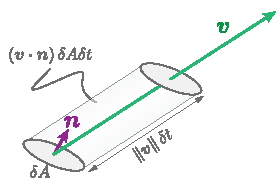
\includegraphics{./pics/slanted_cylinder.pdf}
\caption{A surface portion $\delA$ of normal $\bn$ is traversed by a fluid volume $\lp\bu \!\cdot\!\bn\rp\delA\,\delt$ during $\delt$. This volume is counted positively if  $\bu$ points towards the same half-space as $\bn$ (in which case $\bu \!\cdot\! \bn > 0$), and negatively otherwise.}
\label{fig:slanted_cylinder}
\end{center}
\end{figure}
Now if the surface element is \textbf{mobile} and moves at velocity $\bw$, the advection flux generalises to: 
 \begin{equation}
\bj_\text{adv} = c\, (\bu-\bw)
\end{equation}
We note that in the context of a \textbf{material domain}, i.e. moving with the same velocity as the fluid, we get $\bw = \bu$ and the advection flux cancels out by construction.
\subsection{Diffusion\index{flux!diffusive}}
Now, even without any underlying flow, simple matter (species concentration), energy or momentum inhomogeneities will give rise to transfer spontaneously. These \textbf{diffusive} exchanges are quantified per unit surface and time with the \textbf{diffusive flux}~$\bj_\text{diff}$. 
Even if a detailed modelling of these exchanges is a complex feat, they can nonetheless be described with phenomenological relations (constrained with thermodynamical arguments) such as Fick's law for mass transport for example (see \S\ref{sec:constitutive_laws}).
\section{Balance equation for an integrated quantity\index{conservation law}}
Fluxes characterise exchanges across surfaces. With their help we can determine the evolution of a quantity $c$ contained in a domain in the most general way\footnote{This relation is obtained on \textbf{physical} grounds.}:
\begin{equation}
\underbrace{\vphantom{\oiint_{\partial V}}\dd{}{t}\iiint_{V}c\, \dV}_\text{Variation} = -\underbrace{\oiint_{\partial V} \bj\!\cdot\!\bn\,\dS}_\text{Exchange} + \underbrace{\vphantom{\oiint_{\partial V}}\iiint_{V} \varphi\,\dV}_\text{Production},
\label{eq:conservation_law}
\end{equation}
so that the \textit{variation} of an integrated quantity in  $V$ is given by a balance of entering/leaving quantity into/from the domain (\textit{exchange}) and the possible \textit{production} (or destruction) of $c$ inside $V$.
Before going deeper into the derivation of conservation laws, we have to precise the meaning of the integral derivation appearing in the left hand side. If the considered volume is fixed, the derivation process is easy as we can just swap derivation and integration. But if the domain is moving or deforming, care must be taken in writing this derivation.
\subsection{Volume variation of a material domain and integral derivation}
We will now give a meaning to the derivation of an integral performed over a deformable domain. To start with, let's consider the quite specific (but still really common) case of a \textbf{material} domain, i.e. we follow the same fluid particles though time. As time flows this domain may see its volume change as indicated on figure~\ref{fig:volume_change}, hence as:
\begin{equation}
\dd{}{t}\iiint_{V}\, \dV = \oiint_{\partial V} \bu\!\cdot\!\bn\,\dS \quad \lp = \iiint_V \nabla \!\cdot\! \bu \, \dV\rp.
\end{equation}
\begin{figure}[htbp]
\begin{center}
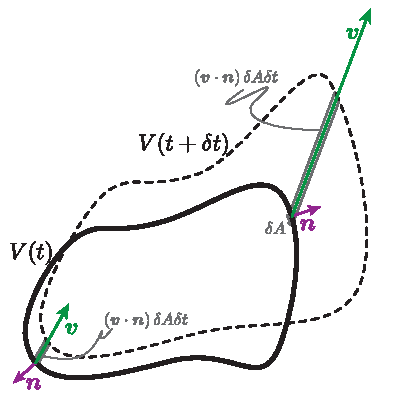
\includegraphics{./pics/volume_change.pdf}
\caption{A material volume is transported by a velocity field $\bu$. Each portion $\delA$ of the domain boundaries is advected with $\bu$ and this yields a volume change $\lp\bu\!\cdot\!\bn\rp\delA\delt$ during $\delt$. The resulting total volume change rate $\dd{V}{t}$ is given by $\iint \lp\bu\!\cdot\!\bn\rp \dA$.}
\label{fig:volume_change}
\end{center}
\end{figure}

\paragraph{$\rhd$ Signification of the divergence.\index{divergence (meaning)}} The previous relation allows to shed light on the divergence of a velocity field~$\bu$. Actually, consider a material volume $\tau(t)$ constituted with the same fluid particles. The previous balance might be rewritten with the help of the divergence theorem as:
\begin{align}
\dd{\tau}{t} &= \iint \bu \!\cdot\! \bn \, \dS\\
		&= \iiint \nabla \!\cdot\! \bu \, \dV.
\end{align}
Thus in the limit where $\tau(t)$ is really small (in fact sufficiently small so that we can consider  $\nabla \!\cdot\! \bu$ constant throughout the domain), we can write:
\begin{equation}
\lim_{\tau \to 0} \frac{1}{\tau} \dd{\tau}{t} = \nabla \!\cdot\! \bu.
\end{equation}
The divergence of a velocity field can therefore be understood as the \textit{rate of volume change of a fluid particle.}
\prg{Integral derivation.} We now have the toolset enabling the clarification of the derivation of the integral over a material domain $V(t)$. Let's focus on the variation of the following quantity:
$$
\dd{}{t} \iiint_{V(t)} \theta \,\dV.
$$
To shed some light over this quantity, let's divide mentally the domain in a multitude of tiny cubes or fluid particles.
As the fluid domain moves, the value of $\theta$ will change for all fluid particles at the rate $\D{\theta}{t}$. Moreover the integration element $\mathrm dV$ will change as well with the rate $\lp\nabla\!\cdot\!\bu\rp\mathrm dV$. In other words\footnote{This relation is obtained on \textbf{mathematical} grounds.}\footnote{We note that this relation can directly be generalised to the case where the domain moves with a velocity differing from that of the fluid (fictitious velocity, flame propagation, balance over a domain moving with a wave). In this case, it suffices to replace $\bu$ with the domain velocity $\bw$.}  :
\begin{equation}
\dd{}{t} \iiint_{V(t)} \theta \,\dV = \iiint_{V(t)} \D{\theta}{t} \,\dV + \iiint_{V(t)} \theta \underbrace{\D{\dV}{t}}_{\lp\nabla \cdot \bu\rp\dV}
\end{equation}
\subsection{Conservation of a quantity. Application to mass conservation}
Now that the derivation of an integral has been elucidated, we are in a position to use equation~(\ref{eq:conservation_law}) which expresses the general conservation of a quantity, for either a fixed or moving domain. Choosing one type of domain or another is largely a matter of context. For example we may consider a moving domain to establish the momentum conservation equation of a given fluid portion. A balance over a fixed domain may also present some interest, when designing for example the evolution of a quantity traversing a fixed mesh cell in a numerical code. Depending on the application, we will choose the more relevant viewpoint.

In order to clarify the use of balances over fixed or moving domains, let's now establish the mass conservation equation (without production nor destruction of mass), first in a fixed domain and then in a moving one.
\begin{enumerate}
\item \textbf{Mass conservation in a fixed domain} $V_\text{fixed}$. The balance equation~(\ref{eq:conservation_law}) reads :
\begin{equation}
\dd{}{t}\iiint_{V_\text{fixed}} \rho \, \dV = - \oiint_{\partial V_\text{fixed}} \rho \bu \!\cdot\! \bn \, \dS.
\end{equation}
The domain being fixed, we let the derivation enter in the integral:
\begin{equation}
\iiint_{V_\text{fixed}} \pd{\rho}{t} \, \dV = - \oiint_{\partial V_\text{fixed}} \rho \bu \!\cdot\! \bn \, \dS,
\end{equation}
and, on applying the divergence theorem, we obtain:
\begin{equation}
\iiint_{V_\text{fixed}} \pd{\rho}{t}  + \nabla \!\cdot\! \lp\rho \bu \rp \, \dV = 0.
\end{equation}
Further noting that this balance is actually true for every possible domain, it follows that the integrand actually vanishes:
\begin{equation}
\pd{\rho}{t}  + \nabla \!\cdot\! \lp\rho \bu \rp = 0.
\label{eq:continuity}
\end{equation}
This is the \textbf{continuity equation\index{conservation law!mass conservation}\index{continuity equation}}\footnote{This denomination has been used for a long time, but is actually not really justifiable\dots} that embodies mass conservation. This type of reasoning exploiting the validity of an integral expression for any volume to obtain a relation at the fluid particle (or \textit{local}) level is very common.
\item \textbf{Mass conservation for a material domain} $V(t)$. This time there is no flux term because no fluid particle enters nor leaves the material domain, by definition. The balance equation~(\ref{eq:conservation_law}) then reads:
\begin{equation}
\dd{}{t}\underbrace{\iiint_{V(t)} \rho \, \dV}_{m(t)} = 0.
\end{equation}
But as the domain is now moving, we have to apply the integral derivation procedure seen earlier:
\begin{equation}
\dd{}{t} \iiint_{V(t)} \rho\, \dV = \iiint_{V(t)} \D{\rho}{t} + \rho \nabla \!\cdot\! \bu\,\dV = 0.
\end{equation}
From the latter we recover again the continuity equation~(\ref{eq:continuity}).
\end{enumerate}
\prg{Conservation of a quantity per unit mass.} Thanks to the continuity relation it is possible to obtain a simplified expression for the transport of a quantity per unit mass $\xi$ (i.e. such that the quantity associated with a fluid particle be $\rho\xi$):
\begin{equation}
\dd{}{t} \iiint_{V(t)} \rho \xi\, \dV = \iiint_{V(t)} \rho \D{\xi}{t} \,\dV.
\end{equation}
We let the reader demonstrate this relation.
\prg{The incompressible fluid.}
A recurring case of great practical value is that of an \textbf{incompressible evolution} where we do \textit{not} suppose that the whole fluid a constant density, but rather that each fluid particle conserves its density. This implies:
\begin{equation}
\D{\rho}{t} = 0 \quad\text{and therefore}\quad \nabla\!\cdot\!\bu=0.
\end{equation}
A velocity field  $\bu$ satisfying the zero divergence property qualifies as a \textit{solenoidal} field.
\subsection{Conservation of a possibly diffusing passive scalar. Convection-diffusion equation}
Let's consider again a concentration field $c$ advected in a fluid domain with the velocity field $\bu$. Due to molecular thermal agitation, this field is also subject to diffusion phenomena characterised by the flux $\bj_\text{diff}$. Here again we can obtain the evolution equation for the concentration by following two different routes:
\begin{enumerate}
\item By considering a \textbf{fixed domain} $V_\text{fixed}$. In this case, and in absence of any source/sink for the concentration, we will simply write that the total variation is given by the sum of the fluxes:
$$
\dd{}{t} \iiint_{V_\text{fixed}} c \, \dV = - \oiint_{\partial V_\text{fixed}} (\bj_\text{conv} + \bj_\text{diff}) \!\cdot\!\bn\,\dS,
$$
so that: 
$$
\iiint_{V_\text{fixed}} \pd{c}{t} \, \dV = - \iiint_{V_\text{fixed}} \nabla \!\cdot\! (\bj_\text{conv} + \bj_\text{diff})\,\dS.
$$
Anticipating on \S \ref{sec:constitutive_laws} by writing the diffusive flux with Fick's law $\bj_\text{diff} = - D \nabla c$ we obtain at the local level:
\begin{equation}
\pd{c}{t} + \nabla \!\cdot\! \lp c\bu\rp = \nabla \!\cdot\! (D \nabla c) 
\label{eq:conv_diff}
\end{equation}
For an incompressible evolution with a constant diffusion coefficient, this equation reduces to the classic \textbf{advection-diffusion equation}:
\begin{equation}
\pd{c}{t} + \lp\bu\!\cdot\!\nabla\rp c = D \nabla^2 c.
\label{eq:conv_diff_incompressible}
\end{equation}
\item Or by considering a \textbf{material domain} $V_\text{mat}$. This time there is no convective flux by construction (see \S\ref{sec:advection}) but only a diffusive flux: 
$$
\dd{}{t} \iiint_{V_\text{mat}} c \, \dV = - \oiint_{\partial V_\text{mat}} \bj_\text{diff} \!\cdot\!\bn\,\dS,
$$
so that, by deriving the integral over the material domain:
$$
\iiint_{V_\text{mat}} \D{c}{t} + c \lp\nabla\!\cdot\!\bu\rp \, \dV = \iiint_{V_\text{mat}} \nabla \!\cdot\! (D \nabla c)\,\dS.
$$
This relation holds true for every possible domain, and as a result we retrieve the local form of equation~$\lp\ref{eq:conv_diff}\rp$.
\end{enumerate}
\subsection{Equation for momentum conservation\index{conservation law!momentum conservation}}
Momentum conservation for a fluid domain simply follows from Newton' second law $m \matrixsym \gamma = \Sigma \matrixsym F$, never forget this!
Let's write this law for a material domain $V(t)$ :
\begin{equation}
\dd{}{t} \iiint_{V_\text{mat}} \rho u_i\,\dV = \oiint_{\partial V_\text{mat}} \sigij n_j\,\dS + \iiint _{V_\text{mat}}\rho F_i \,\dV
\end{equation}
or, going to the local level:
\begin{equation}
\rho \D{u_i}{t} = \pd{\sigij}{x_j} + \rho F_i 
\label{eq:momentum_conservation}
\end{equation}
That was quite simple. However there is a loophole in the previous expression as the stress tensor $\mathsfbfit \sigma$ is here unknown (except in the case of limited interest of a static fluid, see equation \eqref{eq:static_stress_tensor}). Even if equation~\eqref{eq:momentum_conservation} holds true whatever the nature of the fluid (even for say exotic viscoelastic fluids), it is of limited use as long as this stress tensor is not clarified. We therefore have to make a connection between the stresses and the motion of the fluid, for we expect that the stresses will change as soon as the fluid starts to flow. This connection will me be made thanks to \textit{constitutive laws} that will really characterise the fluid we are looking at.

\section{Constitutive laws\index{constitutive laws}}
\label{sec:constitutive_laws}
The conservation laws expressed for a flowing fluid are expressed with fluxes and stresses whose precise form still remains to be determined. In order to make some progress in this determination, let's consider the following situation: without any macroscopic motion, a liquid contains a colourant with concentration $c$ distributed inhomogeneously, with area more or less concentrated. Even in absence of a mean motion, the collisions between molecules will lead the colourant molecules to migrate randomly in the liquid. As a result, due to the inhomogeneous colourant distribution, there will be an excess of particles traversing $\delA$ that originate from a more concentrated area than the reverse. The consequence is a net transport of colourant molecules from more concentrated area to less concentrated ones, that will be active as long as the non-equilibrium situation persists: this is the \textbf{diffusion process}. It seems difficult to track the motion of each colourant particles from a statistical viewpoint. But from a \textit{phenomenological} viewpoint, it is quite clear that diffusion will remain active only if a concentration gradient $\nabla c$ exists. The idea of \textbf{gradient-type laws} is to suppose that the components of the flux $\bj_\text{diff}$\ depend linearly on $\nabla c$, i.e. :
\begin{equation}
\lp \bj_\text{diff}\rp_i = \kij \pd{c}{x_j}.
\end{equation}
For an isotropic fluid, it seems reasonable to consider that in absence of any privileged axes the flux will be aligned with $\nabla c$ and of opposite sign (so as to restore equilibrium rather than to destroy it further!), so that :
\begin{equation}
\bj_\text{diff} = -k \nabla c,
\end{equation}
and therefore:
\begin{equation}
\kij = -k \delij.
\end{equation}
We here recover the general form of mass (Fick) and energy (Fourier) transport:
\begin{empheq}[left=\empheqlbrace]{alignat=2}
&\text{\textbf{Fick}'s law} :\qquad &  \bj_\text{mass} = -D \nabla c\label{eq:fick_flux} \\
&\text{\textbf{Fourier}'s law} :\qquad & \bj_\text{energy} =-k \nabla T\label{eq:fourier_flux}
\end{empheq}
\prg{Momentum diffusion and viscous stress.} The case of momentum diffusion is a bit more complex due to the vectorial nature of $\rho \bu$. To start with let's consider the simple situation of a parallel flow $\lp U(y),0,0\rp$. Due to intermolecular collisions, there is a vertical \textbf{diffusion} of momentum. As for mass transport, we suppose that the flux is linear with the momentum gradient, so that:
\begin{equation}
j_\text{diff} = -\mu \dd{U}{y},
\label{eq:momentum_flux}
\end{equation}
Note that this vertical flux of horizontal momentum has the following dimensions;
$$
\text{momentum per unit volume} \times \text{volume} / \text{area} / \text{time}
$$
or $[\mathsf{ML^{-1}T^{-2}}]$, the same dimension of a stress. This dimensional similitude is no coincidence: the transferred momentum is achieved with a stress, in accordance with Newton' second law. We may indeed rewrite~\eqref{eq:momentum_flux} as:
\begin{equation}
\sigxy = \mu \dd{U}{y},
\label{eq:momentum_flux_stress}
\end{equation}
which is the horizontal stress exerted on a surface with a vertical normal\footnote{the reader will note the sign difference between the expressions~\eqref{eq:momentum_flux} and~\eqref{eq:momentum_flux_stress} that originate from the notation convention for stresses.}. The proportionality coefficient $\mu$ characterising the efficiency of momentum transport is the \textit{dynamic viscosity\index{viscosity}}.
\prg{General expression for the stress tensor of a Newtonian fluid.} In the context of a general flow, we can foresee that the stress tensor will depend on each component of the velocity gradient\footnote{This is this linear dependence to shear that qualifies a fluid as Newtonian. But we can imagine (and actually there exists) more complex relations, of nonlinar nature, between stress and shear. \textbf{Rheology} is the discipline that studies these particular non-newtonian behaviours.}, so that:
\begin{equation}
\sigij = -p \,\delij + \alphaijkl \pd{u_k}{x_l}.
\end{equation}
This form of the stress tensor is compatible with the static fluid stress tensor presented earlier: as soon as the velocity vanishes, the stress tensor adopts its static limit~\eqref{eq:static_stress_tensor}. But we can go further. If we decompose the velocity gradient tensor into a symmetric part \textbf{\textsf{\textit{e}}} (associated with a deformation) and an antisymmetric part $\mathsfbfit \omega$ (associated with solid body rotation) :
$$
u_{i,j} = e_{i,j} + \omega_{i,j} \quad \text{with}\quad 
e_{i,j} = \frac{1}{2}\lp\pd{\vphantom{u_j}u_i}{x_j}+\pd{u_j}{x_i}\rp \quad\text{et}\quad
\omega_{i,j}= \frac{1}{2}\lp\pd{\vphantom{u_j}u_i}{x_j}-\pd{u_j}{x_i}\rp,
$$
Actually momentum diffusion (i.e. viscous stress) can only occur when the flow deviates from solid-body motion (translation or rotation): as a result $\mathsfbfit \sigma$ cannot depend on $\mathsfbfit \omega$ and:
\begin{equation}
\sigij = -p\, \delij + \Aijkl e_{kl}.
\end{equation}
Additional considerations on the fluid isotropy that we will not develop here allow for a drastic reduction in the number of coefficients to finally get:
\begin{equation}
\sigij = -p \,\delij + 2 \mu e_{ij} + \lambda \lp\nabla\!\cdot\!\bu\rp \delij.
\label{eq:newtonian_stress_tensor}
\end{equation}

\section{Navier-Stokes equation}
Having elucidated the structure of the stress tensor~\eqref{eq:newtonian_stress_tensor} we can rewrite the equation for momentum conservation~\eqref{eq:momentum_conservation} :
\begin{equation}
\rho \D{u_i}{t} =  \rho f_i  - \pd{p}{x_i} + \pd{}{x_j} \lp 2 \mu e_{ij} + \lambda \lp\nabla\!\cdot\!\bu\rp \delij \rp
\end{equation}
This equation is the \textit{Navier-Stokes equation}.

In the particular case (but of great practical interest) of an incompressible evolution with viscosity gradient, this equation simplifies to:
\begin{equation}
\rho \D{u_i}{t} =  \rho f_i  - \pd{p}{x_i} + \mu \frac{\partial^2 u_i}{\partial x_j\partial x_j},
\end{equation}
or, in vectorial form:
\begin{equation}
\underbrace{\rho \lp\pd{\bu}{t} + \lp\bu\!\cdot\!\nabla\rp\bu\rp}_{m\matrixsym\gamma} = \underbrace{\vphantom{\lp\pd{\bu}{t}\rp}-\nabla p + \mu \nabla^2 \bu + \rho \bff}_{\Sigma \bF}.
\end{equation}

%\section{Mini-projet : sur l'intérêt de l'adimensionnement}
%Manip parachute

% !TEX root = ./physics_of_fluids.tex
% !TEX TS-program = xelatex
% !TEX encoding = UTF-8 Unicode
\chapter{Boundary conditions and interfaces}
\label{chap:boundary_conditions}
We have seen in the previous chapter how to express mass and momentum conservation at the fluid particle level, and we have derived the corresponding equations for fluid motion. These equations are naturally associated with \textbf{boundary conditions} that either express conservation laws (e.g. no mass flux at a boundary) or peculiar physical processes occurring at a surface (temperature or velocity continuity). In both cases these boundary conditions will be pivoting in the determination of the solution.
%\section{Flux aux frontières : imperméabilité et imbibition}
%\begin{figure}[htbp]
%\begin{center}
%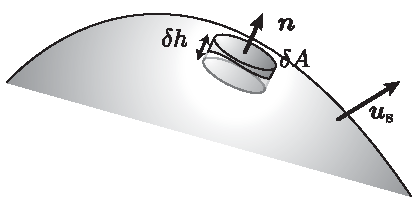
\includegraphics{./chapters/pics/impermeability.pdf}
%\caption{On effectue un bilan sur un volume élémentaire situé à cheval sur la frontière solide.}
%\label{fig:impermeability}
%\end{center}
%\end{figure}
%
%Considérons un solide se déplaçant dans un fluide à la vitesse $\bu_\text s$ (éventuellement dépendante du temps) et effectuons un bilan de masse sur un petit volume cylindrique de base $\delA$ et de hauteur $\delh$ à cheval entre le fluide et le solide (Fig.~\ref{fig:impermeability}). Faisons maintenant tendre $\delh$ vers 0 de sorte à ce que l'élément ait une masse nulle. Ainsi, la variation de masse de l'élément est nécessairement zéro, ce qui veut dire que le flux de masse du côté fluide doit être équilibré par le flux de masse du côté solide :
%\begin{equation}
%-\lp\bj_\text{fluide}\cdot \bn_\text{fluide}\rp \delA -  \lp\bj_\text{solide}\cdot \bn_\text{solide}\rp \delA = 0.
%\end{equation}
%Posons arbitrairement $\bn = \bn_\text{fluide} = - \bn_\text{solide}$, il vient :
%\begin{equation}
%-\bj_\text{fluide}\cdot \bn +  \bj_\text{solide}\cdot \bn = 0.
%\end{equation}
%En l'absence d'effets de mélange, la vitesse $\bu$ du fluide tient compte des effets diffusifs (il s'agit de la vitesse de l'espèce) et le flux de masse se résume au flux convectif. Attention : comme nous nous plaçons dans le référentiel du solide, la vitesse relative du fluide est $\bu - \bu_\text s$, de sorte que le flux de masse du côté fluide s'écrive :
%\begin{equation}
%\bj_\text{fluide} = \rho \lp\bu-\bu_\text s\rp.
%\end{equation}
%\prg{La paroi imperméable.} Un cas de figure extrêmement courant est celui d'un solide \textbf{imperméable}, c'est-à-dire dans lequel le fluide ne peut pénétrer ; le flux de masse de fluide dans le solide est alors nul et on a $\bj_\text{solide} = \boldsymbol 0$. La conservation de la masse exprimée à la frontière d'une telle paroi imperméable se réduit alors à :
%\begin{equation}
%\bu\cdot\bn = \bu_\text s \cdot\bn
%\label{eq:impermeabilite}
%\end{equation}
%C'est la \textbf{condition d'imperméabilité} d'un objet (ou d'une paroi), qui comme son nom l'indique, traduit simplement le fait que le fluide ne pénètre pas le solide et qui s'exprime par la \textbf{continuité des vitesses normales}.
%
%Note : dans le cas particulier (mais très courant !) d'une objet solide fixe, cette condition devient  $\bu\cdot\bn =0$.
%\prg{Paroi perméable.} La discussion précédente s'étend naturellement au cas des parois perméables. Celles-ci peuvent correspondre à des tissus biologiques perméables à certains solutés, à des matériaux pouvant être imbibés par des solvants, des terrains trempés par la pluie ou encore des profils portants percés à des fins de contrôle de couche limite (comme la turbovoile de Cousteau et Malavard illustrée dans la séquence vidéo du cours).
%
%Le flux de masse au sein de la paroi n'est désormais plus nul et sa détermination requiert de connaître le type d'écoulement au sein du solide. Supposons toutefois la vitesse d'imbibition $\bu_\text{imbib}$ constante et connue (correspondant par exemple au cas d'une aspiration à débit imposé). La conservation de la masse à une paroi perméable mobile s'écrira alors :
%\begin{equation}
%\rho (\bu-\bu_\text s) \cdot \bn = \rho (\bu_\text{imbib}) \cdot \bn,
%\end{equation}
%soit 
%\begin{equation}
%\bu\cdot\bn = \lp\bu_\text s + \bu_\text{imbib}\rp\cdot\bn.
%\end{equation}
%\prg{Condition limite sur un champ de concentration à une paroi.}
%Les conditions limites à appliquer sur l'équation de transport d'un champ de concentration~(\ref{eq:conv_diff}) peuvent être obtenues suivant le même principe. Imaginons pour cela un champ de concentration transporté par un écoulement $\bu$ au sein duquel un solide (imperméable) se meut à la vitesse $\bu_\text s$. Dans le référentiel du solide le flux de matière à travers une surface $\delA \,\bn$ quelconque est :
%\begin{equation}
%\bj_\text{matière} = \bj_\text{conv} + \bj_\text{diff} = c \lp \bu - \bu_s\rp - D \nabla c.
%\end{equation}
%La condition d'imperméabilité de la paroi au champ de concentration $c$ s'écrit donc :
%\begin{equation}
%c (\bu-\bu_\text s) \cdot \bn - D \nabla c \cdot \bn = 0,
%\end{equation}
%car le flux de matière est nul dans le solide.
%En utilisant la condition d'imperméabilité du champ de vitesse~(\ref{eq:impermeabilite}), cette relation se réduit à :
%\begin{equation}
%\nabla c \cdot \bn \equiv \pd{c}{n} = 0.
%\end{equation}
%\prg{Transfert de masse à une interface : évaporation.} Un dernier exemple d'obtention de conditions limites à partir d'une équation de bilan est la condition de continuité du flux de masse à travers une interface liquide-gaz, dans le cas où le liquide s'évapore. 
%
%Effectuons un bilan de masse sur le même type d'élément de volume que celui considéré précédemment : un petit élément cylindrique de base $\delA$ et de hauteur $\delh$ à cheval sur l'interface se déplaçant à $\bu_\text i$. On fait tendre la hauteur $\delh$ de l'élément vers 0, de sorte à ce que la masse de l'élément tende vers 0 également. Le bilan de masse sur cet élément s'écrit :
%\begin{equation}
%\bj_\text{conv. liquide} = \bj_\text{conv. gaz} + \bj_\text{diff. gaz}
%\end{equation}
%soit :
%\begin{equation}
%\rho_\ell \lp\bu_\ell - \bu_\text i\rp \cdot \bn = \rho_v \lp\bu_g -\bu_\text i\rp\cdot \bn - D \nabla \rho_v \cdot n
%\end{equation}
%Si l'évaporation est très violente (e.g. front de combustion), le flux est dominé par les effets de convection et 
%$$\bu_g \sim \underbrace{\frac{\rho_\ell}{\rho_v}}_{\gg 1} \bu_\ell$$
%c'est-à-dire que l'écoulement (dit de Stefan) induit dans la vapeur est beaucoup plus violent que celui dans le liquide.
%Dans l'autre limite, où l'évaporation est très lente (cas d'une goutte d'eau séchant librement), c'est plutôt le terme diffusif qui domine.
%\section{Conditions phénoménologiques : adhérence aux parois et continuité}
%En plus des conditions précédentes découlant de principes de conservation, les fluides sont sujets à d'autres conditions limites, établies et confirmées sur des bases expérimentales et faisant l'objet d'un consensus, mais pas d'un démonstration exacte. Ces conditions phénoménologiques sont les conditions de \textbf{continuité des champs} aux interfaces, comme la vitesse, la température etc.
%
%\paragraph{$\rhd$ Une brève histoire de l'adhérence.} La condition d'adhérence, $\bu = \bu_\mathrm{s}$, a une histoire étonnante et pleine de rebondissements, dont nous traçons les grandes lignes dans ce qui suit \citep{Goldstein1950}. Au \textsc{XVIII}$^e$ siècle, la description théorique des écoulements potentiels (correspondant à l'approximation d'écoulement parfait de fluide) était déjà bien place, mais les comparaisons avec les expériences étaient médiocres. Daniel Bernoulli en était bien conscient et attribuait les différences entre les écoulements (parfaits) prédits et ceux observés expérimentalement à une ``condition d'adhérence'' qui devait prévaloir aux parois. Coulomb démontra par la suite expérimentalement qu'un disque oscillant dans un liquide ne semblait pas particulièrement affecté par un changement de ses propriétés de surface (lisse, rugueuse ou recouverte de graisse), si bien qu'il lui semblait également que la vitesse de l'écoulement correspondait à celle du disque. Dans cette vision, le fluide a les mêmes propriétés en tout point de l'espace, et il satisfait simplement une condition additionnelle à la paroi.
%
%Mais au cours du \textsc{XIX}$^e$ siècle des théories concurrentes sont apparues. Girard proposa ainsi que la couche liquide touchant la paroi avait des propriétés physiques différentes l'amenant à adhérer au solide. La couche directement adjacente (composée de fluide ``normal'') pouvait quant à elle glisser parfaitement sur la première. Navier s'intéressa également au problème et avança une condition limite impliquant un glissement proportionnel à la contrainte de cisaillement $\beta u = \mu \pd{u}{n}$, où le ratio $\mu/\beta$ a la dimension d'une longueur : la \textit{longueur de glissement}. Il s'en suivit une période de relative confusion, où les grands théoriciens de l'époque (Poisson, Stokes) ont adopté alternativement l'une ou l'autre des conditions limites.
%
%Au fil du temps cependant, des expériences fines conduites notamment par Couette ou Maxwell firent définitivement pencher la balance du côté de la condition d'adhérence. Maxwell suggéra sur des considérations moléculaires que si la condition de Navier est bien à l'\oe uvre, la longueur sur laquelle s'effectue le glissement est si petite -- de l'ordre de quelques libre-parcours moyens -- qu'il est très raisonnable de la considérer nulle, i.e. de considérer adhérence à la paroi : $\bu = \bu_\text s$. Ceci est en particulier respecté dans les conditions usuelles des expériences et laboratoires, mais pas nécessairement dans des conditions de gaz raréfiés (e.g. rentrée dans l'atmosphère, vol hypersonique) ou d'écoulements de longues chaînes de polymères (écoulements en piste microfluidique), comme le confirment les expériences.
%
%Au \textsc{XX}$^e$ siècle, l'accord quasiment parfait entre les observations expérimentales et la prédiction utilisant la condition d'adhérence pour de nombreux écoulements, comme l'écoulement de Poiseuille, de Couette, la chute de la sphère de Stokes en fluide visqueux, le seuil d'instabilité dans l'expérience de Taylor-Couette... ont définitivement convaincu de la validité de cette condition. 
%
%Par ailleurs, les lois d'échelle sur la traînée d'un objet déduites de l'analyse dimensionnelle sur la base des échelles caractéristiques $\rho, U, D$ et $\mu$ capturent l'évolution des efforts aérodynamiques sur une vaste plage d'échelles. Si une autre échelle de longueur (associée au glissement à la paroi) était pertinente dans la description des écoulements, les lois d'échelles s'en trouveraient modifiées. 
%
%On peut comprendre cette condition d'adhérence (continuité de $\bu$ de part et d'autre de l'interface) tout comme la condition de continuité des températures comme résultant d'équilibre à l'échelle moléculaire : les transferts extrêmement rapides entre molécules adjacentes induisent l'équilibrage instantané de la quantité de mouvement moyenne (vitesse) et de la vitesse d'agitation thermique (température) \citep{Batchelor1967}. À une interface entre un milieu I et un milieu II (solide-fluide, ou fluide-fluide), on aura donc :
%\begin{equation}
%\bu_\text I = \bu_\text{II} \quad \text{et} \quad T_\text I = T_\text{II}
%\end{equation}

\bibliographystyle{jfm}
\bibliography{biblio_pof}
\printindex
\end{document}
